\documentclass{beamer}
\usepackage[utf8]{inputenc}
\usepackage{graphicx}
\usetheme{default}
\usecolortheme{default}

\title[S02 Régression et MCO]{Section 04 : Les modèles panels\\ (Séance 8)}
\subtitle{GSF-6053: Économétrie Financière}
\author[SP. Boucher]{Simon-Pierre Boucher\inst{1}}
\institute[Université Laval]
{
  \inst{1}%
  Département de finance, assurance et immobilier\\
  Faculté des sciences de l'administration\\
  Université Laval}
\date[Hiver 2022]{15 Mars 2022}

\begin{document}

\begin{frame}
  \titlepage
\end{frame}

\begin{frame}{Références}
\textbf{Obligatoires:}
\begin{itemize}
\item \textbf{Notes de cours:} Section 2 (Professeure: Marie-Hélène Gagnon)
\item \textbf{Woolridge:} chapitres 13 et 14.
\end{itemize}
\vspace{0.5cm}
\textbf{Complémentaires:}
\begin{itemize}
\item \textbf{Gujarati et Porter:} chapitre 16
\end{itemize}
\end{frame}

\begin{frame}{Plan de la séance}
  \tableofcontents
\end{frame}

\section{Les modèles panels}
\frame{\tableofcontents[current]}
\begin{frame}{Les modèles panels}
\begin{itemize}
\item Il est possible de faire des estimations multivariées où $Y$ est une matrice $T \times n$.
\item Par exemple, nous pourrions vouloir estimer le modèle du CAPM sur plusieurs actifs à la fois. 
\item Au lieu de faire une série de régressions séparées sur plusieurs actifs financiers, nous formerons un système d’équations multivariées.
\item Cette approche permet plusieurs innovations dans la modélisation qui peuvent être intéressantes :
\begin{itemize}
\item Comparaison statistique de coefficients entre équations d’un même système.
\item Test conjoint des implications du modèle (telle que l’efficacité moyenne-
variance) sur plusieurs portefeuilles ou actifs financiers.
\item Permets une plus grande flexibilité au niveau de la modélisation du terme
d’erreur des équations du système.
\end{itemize}
\end{itemize}
\end{frame}

\begin{frame}{Les modèles panels}
\begin{block}{Le CAPM univarié}
\begin{align*}
R_{t}-R_{Ft}=\alpha+\beta (R_{Mt}-R_{Ft})+U_{t}
\end{align*}
\end{block}
\begin{block}{Le CAPM multivarié}
\begin{align*}
R_{\textbf{j}t}-R_{Ft}=\alpha_{\textbf{j}}+\beta_{\textbf{j}} (R_{Mt}-R_{Ft})+U_{\textbf{j}t}
\end{align*}
\begin{itemize}
\item $R_{\textbf{j}t}-R_{Ft}$ représente le rendement excédentaire au temps $t$ de l'actif $j$ par rapport à un titre sans risque.
\item On cherche a expliquer le rendement excédentaire du titre $j$ avec la prime de risque du marché $R_{Mt}-R_{Ft}$.
\item $\alpha_{\textbf{j}}$ est une constante et $\beta_{\textbf{j}}$ mesure la sensibilité du rendement excédentaire de l'actif $j$ au rendement excédentaire du marché.
\end{itemize}
\end{block}
\end{frame}


\begin{frame}{Les modèles panels}

\begin{block}{Le CAPM multivarié}
\begin{itemize}
\item Selon le CAPM, les interceptes d’un modèle en rendements excédentaires devraient être nulles (hypothèse d’efficience moyenne variance).
\begin{itemize}
\item $\alpha_{\textbf{j}}=0$ 
\end{itemize}
\item $t=1,\cdots, T$ représente l'indicateur temporelle. Pour chaque actif, nous aurons T rendement, allant de $t=1$ jusqu'à $t=T$
\item $j=1, \cdots,N$ représente l'indicateur du titre ou portefeuille. Dans notre modèle univarié, nous aurons $N$ titres ou portefeuilles.
\item Nous n’avons pas encore spécifié la forme du terme d’erreur $u_{\textbf{jt}}$ 
\end{itemize}
\end{block}
\end{frame}

\begin{frame}{Les modèles panels}
\begin{itemize}
\item Typiquement dans le cadre des données panel nous aurons deux éléments:
\begin{itemize}
\item Plusieurs individus ou portefeuilles ou groupe (N)
\item Quelques observations temporelles (T)
\end{itemize}
\item Un exemple de données panels serait des données sur
\begin{itemize}
\item l’investissement (I)
\item la valeur de la firme (F) 
\item la capital (C)
\item pour 20 années
\item Données sur les investissements de quatre entreprises \textbf{(Table 1.2 dans Gujarati et Porter.)}
\end{itemize}
\end{itemize}
\end{frame}


\begin{frame}{Les modèles panels}
\begin{block}{Données sur les investissements de quatre entreprises}
\begin{center}
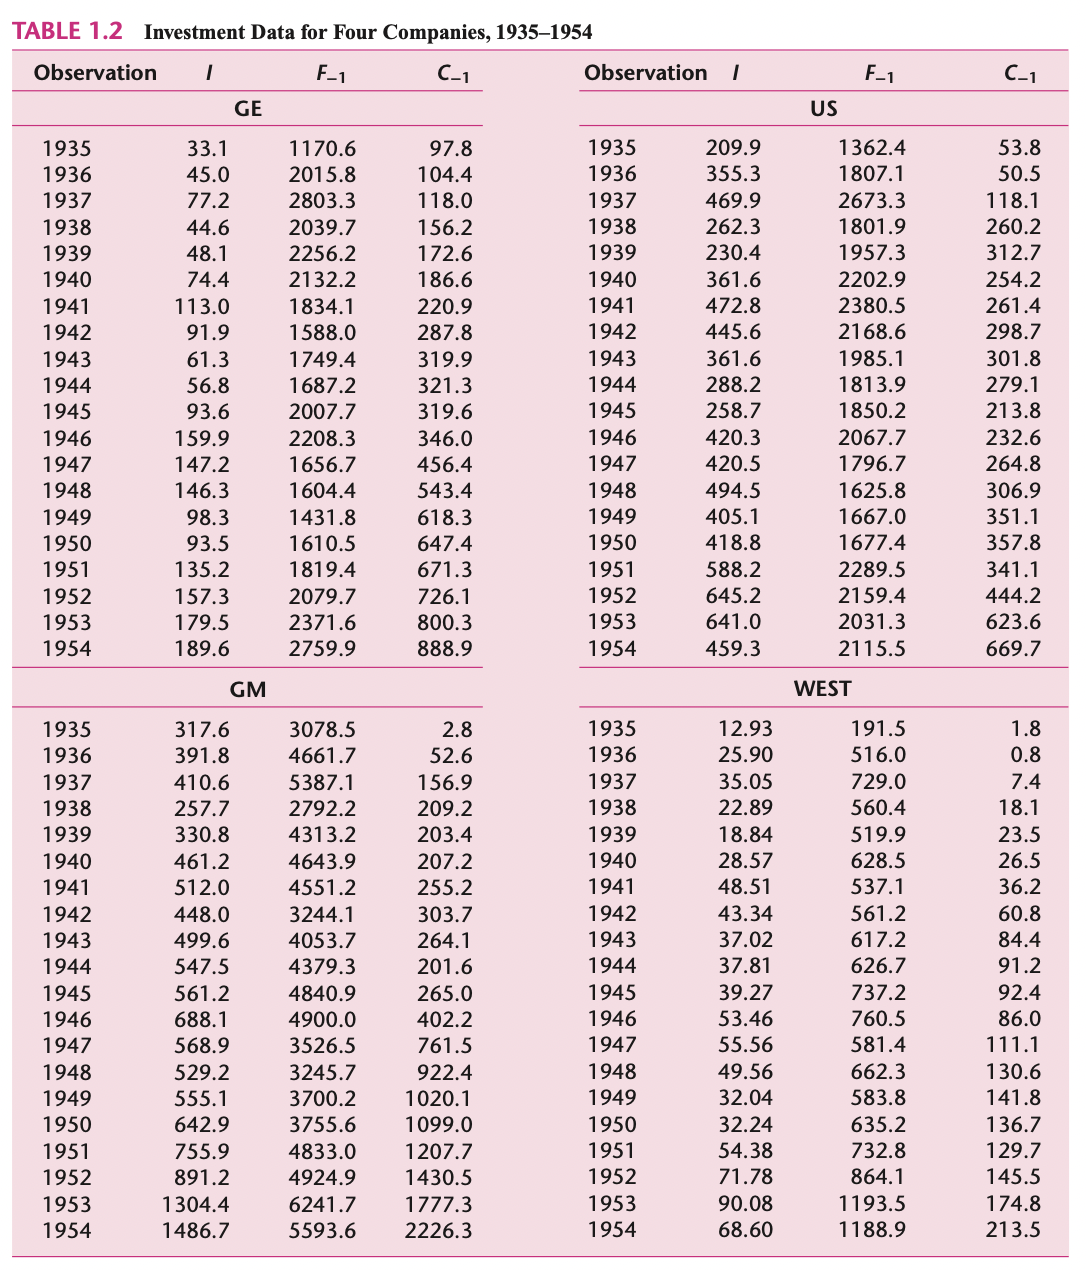
\includegraphics[scale=.3]{ex1.png}
\end{center}
\end{block}
\end{frame}

\begin{frame}{Les avantages des données panel}
\begin{itemize}
\item Permet de tenir compte de l’hétérogénéité entre les groupes (ou portefeuilles, etc.) en définissant des variables \textbf{sujet-spécifiques}.
\item Les variables sont plus riches et informatives puisqu’elles contiennent plus de variabilité, possiblement moins de colinéarité et permettent plus de degrés de liberté dans les estimations $(T \times N)$


\end{itemize}
\end{frame}

\section{Les avantages des données panel}
\frame{\tableofcontents[current]}
\begin{frame}{Les avantages des données panel}
\begin{itemize}
\item Certains sujets sont plutôt conçus pour les données panels : 
\begin{itemize}
\item Étude de l’emploi en économie ou des habitudes de consommation d’électricité par exemple. 
\item En finance, plusieurs sujets en finance corporative et comptabilité (où les données sont souvent en fréquence annuelle) permettent d’évaluer la valeur de la firme en fonction de données comptables.
\end{itemize}
\item Donne une dimension supplémentaire aux coupes transversales ou aux séries chronologiques.
\item Permet d’agréger de l’information diffuse et de minimiser les biais dus à des agrégations trompeuses (en permettant l’hétérogénéité).

\end{itemize}
\end{frame}

\section{Notation générale pour ces modèles panels}
\frame{\tableofcontents[current]}
\begin{frame}{Notation générale pour ces modèles panels}
\begin{align*}
Y_{it}=X_{it}^{'}\beta + Z_i^{'}\alpha+u_{it}
\end{align*}
\begin{align*}
Y_{it}=X_{it}^{'}\beta +c_i+u_{it}
\end{align*}
\begin{itemize}
\item Où les régresseurs dans X n’incluent pas de constante.
\item L’hétérogénéité vient de $Z_i^{'}\alpha$ où $Z_i^{'}$ contient un terme constant et une série de variables spécifiques au groupe (ou l’individu) i et constante dans le temps.
\begin{itemize}
\item Celles-ci pouvant être soient observées ou non observées.
\item La formulation de $Z_{i}^{'}$ change le modèle adopté.
\end{itemize}
\end{itemize}
\end{frame}

\section{Exemple de données panels}
\frame{\tableofcontents[current]}
\begin{frame}{Exemple de données panels}
\begin{itemize}
\item On analyse des données sur les coûts de six compagnies aériennes pour la période 1970-1984, pour un total de 90 observations de données de panel.
\begin{itemize}
\item $I=$ identifiant de la compagnie aérienne (1 à 6 car 6 firmes)
\item $T=$ l’année (15 années de données)
\item $Q=$ Output (en mile-passagers)
\item $C=$ cout
\item $PF=$ prix de l’essence
\item $LF=$ l’utilisation moyenne des avions, load factor
\end{itemize}
\item Nous avons ici un panel balancé, car le nombre d’observations pour chaque firme est le même.
\item Nous pourrions ajuster l’approche pour des panels non balancés. 
\item C’est aussi ce qu’on appelle un panel long, puisque T est plus grand que n. 
\item Un panel court serait un panel où n est plus grand que T.
\end{itemize}
\end{frame}


\begin{frame}{Exemple de données panels}
\begin{itemize}
\item Nous voulons trouver comment la fonction de coût des compagnies aériennes évolue en fonction de Q, PF, LF.
\item La première approche serait de trouver par OLS 6 fonctions de coût une pour chaque compagnie.
\begin{itemize}
\item Cela néglige de l’information, car celle-ci doit être semblable dans chaque compagnie.
\item Nous aurons peu d’observations pour chaque firme (15) ou alors très peu d’observation par coupe transversale (6) par année. Dans les deux cas, soit on
\item Ignore la dynamique dans le temps (coupe transversale) soit on ignore l’industrie (série chronologique).
\end{itemize}

\end{itemize}
\end{frame}

\begin{frame}{Exemple de données panels}
\textbf{4 options se proposent à nous:}
\begin{block}{1-Modèle pooled}
\begin{itemize}
\item Mettre toutes les observations ensemble et faire une seule estimation OLS sur $T \times n=90$ observations sans s’occuper de la nature des données.
\end{itemize}
\end{block}
\begin{block}{2-Modèle LSDV}
\begin{itemize}
\item Mettre toutes les observations ensemble $T \times n=90$ observations, mais on permet de l’hétérogénéité dans la fonction de cout en fonction de la compagnie aérienne. 
\item Nous permettrons à chaque compagnie aérienne d’avoir un intercepte propre à lui même.
\end{itemize}
\end{block}
\end{frame}


\begin{frame}{Exemple de données panels}
\textbf{4 options se proposent à nous:}
\begin{block}{3-Modèle à effet fixe}
\begin{itemize}
\item On exprime chaque variable en déviation par rapport à sa moyenne de \textbf{groupe} (ici la compagnie aérienne).
\item On explique donc les variations
dans la fonction de cout à l’intérieur d’un groupe \textbf{(within group effect)}
\end{itemize}
\end{block}
\begin{block}{4-Modèle à effet aléatoire}
\begin{itemize}
\item Où les effets de groupe ne sont pas corrélés avec les régresseurs.
\item L’impact du groupe est donc à modéliser dans le terme d’erreur.
\end{itemize}
\end{block}
\end{frame}


\section{Le Modèle pooled}
\frame{\tableofcontents[current]}
\begin{frame}{Le Modèle pooled}
\begin{itemize}
\item Si $Z_{i}^{'}$ contient seulement un terme constant (le même pour tous les groupes), alors les moindres carrés ordinaires nous donneront des estimateurs convergents de $\alpha$ et $\alpha$.
\item L’hypothèse de base de ce cas est qu’il n’y a pas d’hétérogénéité dans les groupes $i$ et il est pertinent d’avoir un estimateur conjoint.
\end{itemize}
\end{frame}

\begin{frame}{Le Modèle pooled}
\begin{itemize}
\item Le modèle aura la forme suivante:
\begin{align*}
Y_{it}=\alpha+\beta' X_{it}+u_{it}
\end{align*}
\begin{itemize}
\item Les erreurs sont indépendantes, d’espérance nulle et de variance $\sigma_u^2$.
\item Les régresseurs $u$ sont toujours strictement exogènes et non corrélés avec le terme d’erreur.
\item C’est le modèle qui représente la moyenne de la population, étant donné ces coefficients contraints. 
\item Les estimateurs MCO sont convergents. 
\end{itemize}
\end{itemize}
\end{frame}

\section{Le modèle avec effets fixes}
\frame{\tableofcontents[current]}
\begin{frame}{Le modèle avec effets fixes}
\begin{itemize}
\item Soit le modèle de base avec les caractéristiques inobservables de chaque groupe $i$:
\begin{align*}
Y_{it}=\beta'X_{it}+c_i+u_{it}
\end{align*}
\item On fait l’hypothèse que les $c_i$ sont correlés avec les régresseurs.
\item Dans ce cas, nous savons que les estimateurs OLS seront biaisés. 
\end{itemize}
\end{frame}


\begin{frame}{Le modèle avec effets fixes}
\begin{itemize}
\item On règle cette question en ajoutant une constante propre à chaque groupe qui représente tous les effets observables du groupe $i$.
\begin{align*}
Y_{it}=\beta'X_{it}+\alpha_i+u_{it}
\end{align*} 
\item Si la variance conditionnelle au régresseur des $c_i$ est constante, ce modèle devient une régression linéaire classique.
\item On appelle cette formulation le modèle avec effet fixe puisqu’il implique que la différence entre les groupes peut être capturée par la différence dans le terme constant. 
\end{itemize}
\end{frame}


\section{Least square dummy variable model}
\frame{\tableofcontents[current]}
\begin{frame}{Least square dummy variable model}
\begin{itemize}
\item Si le nombre de groupe n’est pas trop grand par rapport au nombre d’observations (si vous avez un panel très long).
\item Le modèle peut être estimé par moindres carrés avec le LSDV, Least square dummy variable model où les $\alpha_i$ sont libres.
\item L’idée est des générer des variables dichotomiques $D_i$ qui prennent la valeur 1 quand nous sommes dans le groupe $i$ et zéro sinon.
\end{itemize}
\end{frame}

\begin{frame}{Least square dummy variable model}
\textbf{Modèle LSDV:}
\begin{align*}
y=X \beta + D \alpha +u 
\end{align*}
\begin{itemize}
\item $y$ est un vecteur $(NT \times 1)$
\item $X$ est une matrice $(NT \times k)$
\item $D$ est une matrice $(NT \times N)$
\item On empile les $Y$ dans un grand vecteur $y$. 
\item On empile également les régresseurs un par dessus les autres dans le même ordre et on fait de même avec les variables dichotomiques.
\end{itemize}
\end{frame}

\begin{frame}{Least square dummy variable model}
\textbf{Variable dichotomiques:}
\begin{align*}
D=\begin{bmatrix} 
d_1 & d_2 & \cdots & d_N
\end{bmatrix} 
\end{align*}
\begin{itemize}
\item Sachant que $d_1$, $d_2$ et $d_N$ sont tous des vecteurs $NT \times 1$
\item Les $y$ sont définis selon le modèle empilé et $d_i$ est un vecteur composé de zéros partout sauf pour indiquer le groupe $i$.
\end{itemize}
\textbf{Vecteur $\alpha$: $(N \times 1)$}
\begin{align*}
\alpha=\begin{bmatrix} 
\alpha_1 \\
\alpha_2 \\
\vdots \\
\alpha_N
\end{bmatrix} 
\end{align*}
\end{frame}

\begin{frame}{Least square dummy variable model}
\textbf{Matrice $X$: $(NT \times K)$}
\begin{align*}
X=\begin{bmatrix} 
X_1 \\
X_2 \\
\vdots \\
X_N
\end{bmatrix} 
\end{align*}
\textbf{Vecteur $u$: $(NT \times 1)$}
\begin{align*}
u=\begin{bmatrix} 
u_1 \\
u_2 \\
\vdots \\
u_N
\end{bmatrix} 
\end{align*}
\end{frame}

\begin{frame}{Least square dummy variable model}
\begin{itemize}
\item On estime ce modèle par OLS sur toutes les observations $(NT)$.
\item Pour trouver un estimateur de la variance, on obtient le vecteur de dimension $(NT \times 1)$ des résidus qu’on notera $\hat{u}$.
\item L’estimé de la variance pour le terme d’erreur (bruit blanc) est donc :
\begin{align*}
\hat{\sigma}_u^2=\frac{\hat{u}^{'}\hat{u}}{NT-N-K}
\end{align*}
\end{itemize}
\end{frame}

\begin{frame}{Least square dummy variable model}
\begin{block}{Dummy variable trap}
\begin{itemize}
\item Vous ne pouvez pas inclure une dummy pour chaque groupe si vous voulez avoir une constante au modèle.
\item Si vous voulez une constante dans le modèle, il faut laisser tomber une des dummy et l’utiliser comme point de référence.
\item Supposons que le groupe 1 est votre groupe de référence et que vous incluez une constante.
\begin{itemize}
\item La constante du modèle est l’effet du groupe 1 
\item Les coefficients $\alpha_i$ pour les dummy sont la différence entre le groupe 1 et le groupe $i$. 
\item  Pour avoir l’effet du groupe n par exemple, il faudra additionner les deux:
\begin{align*}
\textbf{cts}+\alpha_n
\end{align*}
\end{itemize}
\end{itemize}
\end{block}
\end{frame}


\end{document}